\documentclass[a4paper,11pt,twoside]{report}
\overfullrule=5pt

\usepackage[
	%showframe, % show frame for page margins etc.
	scale=0.75, % fraction of page width/height to use
	headheight=30pt,
]{geometry}

%\usepackage[utf8]{inputenc} % ignored with lualatex / xelatex (which are utf8-based)
\usepackage{amsmath}
\usepackage[text]{esdiff} % text-mode derivatives in textstyle
\usepackage{tensor}
\usepackage[parfill]{parskip} % new paragraph: new line, no indent
\usepackage[title]{appendix}
\usepackage[hidelinks]{hyperref} % hide colored boxes around links
\usepackage[noabbrev]{cleveref}
\usepackage[labelfont=bf]{caption} % figure title in bold

\usepackage{unicode-math} % make code display utf8 characters properly
\usepackage[cache=false]{minted}
%\setmonofont{DejaVu Sans Mono} % will affect whole document, including URLs etc.
\newfontfamily\codefont{DejaVu Sans Mono}[NFSSFamily=CodeFamily] % set mono font for minted code only
\setminted{breaklines}
\setminted{frame=single}
\setminted{breakanywhere}
\setminted{fontfamily=CodeFamily}

\usepackage{fancyhdr}
\pagestyle{fancy}
\fancyhf{}
\fancyhead[LE,RO]{\textbf{\thepage}}
\fancyhead[RE]{\leftmark}
\fancyhead[LO]{\rightmark}
\fancyfoot[CE,CO]{}

\usepackage{pgfplots}
\pgfplotsset{compat=1.17}
\usepgfplotslibrary{groupplots}

%\fancypagestyle{plain}{\pagestyle{fancy}} % make chapter front pages, bibliography etc. use same style as other pages (see https://tex.stackexchange.com/a/10046)

% make consistent style also on chapter first pages, bibliography etc.
\fancypagestyle{plain}{
	\fancyhf{}
	\fancyhead[LE,RO]{\textbf{\thepage}}
}

\usepackage[style=alphabetic]{biblatex}
\addbibresource{project.bib}

\newcommand\dif{\mathop{}\!\mathrm{d}}
\newcommand{\abs}[1]{\lvert #1 \rvert}
\newcommand{\integral}[4]{\int_{#3}^{#4} #1 \dif #2}

% useful intro to Latex thesis: https://www.overleaf.com/learn/latex/How_to_Write_a_Thesis_in_LaTeX_(Part_1):_Basic_Structure

\title{Project thesis}
\author{Herman Sletmoen}
\date{\today}

\begin{document}

\maketitle

\tableofcontents

\chapter*{Notation and conventions} % do not number
\addcontentsline{toc}{chapter}{Notation and conventions} % but still display in TOC (see https://tex.stackexchange.com/a/222961)
%\markboth{NOTATION AND CONVENTIONS}{} % but still display correct header (see https://tex.stackexchange.com/a/78090)

\section*{Metric signature}

We use the $(-,+,+,+)$ metric signature.

\section*{Units}

We use natural units in which the speed of light $c = 1$.

\section*{Summation convention}

We use the Einstein summation convention, in which an index that appears once as a superscript and again as a subscript in the same term is to be summed over.
If the index is roman, the sum runs from $1$ to $3$, and if it is greek, it also runs over $0$.
For example,
\begin{equation*}
	T\indices{^\mu_\mu} = \sum_{\mu=0}^3 T\indices{^\mu_\mu}
	\quad \text{and} \quad
	T\indices{^i_i} = \sum_{i=1}^3 T\indices{^i_i}
	.
\end{equation*}

\chapter{Tolman-Oppenheimer-Volkoff equation}

TODO: write intro after I know everything we should do in this section

TODO: add page numbers to citations

\section{Derivation from the Einstein field equations}

To analyze astrophysical objects like stars, it is of considerable interest to relate the pressure $p(x)$ and energy density $\epsilon(x)$ at every position $x$ inside the object.
We will derive the relativistic relation between these quantities from the \textbf{Einstein field equations} \cite[equation 4.44]{ref:carroll}
\begin{equation}
	G\indices{_\mu_\nu} = R_{\mu \nu} - \frac{1}{2} R g_{\mu \nu} = 8 \pi G T_{\mu \nu} ,
	\label{eq:einstein}
\end{equation}
It describes how the geometry of spacetime, described by the Ricci tensor $R\indices{_\mu_\nu}$ and Ricci scalar $R$ that are ultimately built from the metric $g\indices{_\mu_\nu}$ and encapsulated in the Einstein tensor $G\indices{_\mu_\nu}$ (see \cref{chap:gr_summary} for a summary), responds to the presence of energy-momentum in the energy-momentum tensor $T\indices{_\mu_\nu}$.
Here, $G$ is the gravitational constant.

Unless rotating very fast, stars are well approximated by spheres.
For our purposes, we therefore consider the most general line element that exhibits spherical symmetry, namely \cite[§ 94-95]{ref:tolman}
TODO: do more general with $\gamma(r)$, as done in Carroll?
\begin{equation}
	\dif s^2 = -e^{2 \alpha(r)} \dif t^2 + e^{2 \beta(r)} \dif r^2 + r^2 \left( \dif \theta^2 + \sin^2 \theta \dif \phi^2 \right) .
\end{equation}

We model the interior of the star as a perfect fluid with energy-momentum \cite[equation 1.114]{ref:carroll}
\begin{equation}
	T\indices{_\mu_\nu} = (\epsilon+p) U_\mu U_\nu + p g\indices{_\mu_\nu}.
\end{equation}
For a static star whose fluid is at rest, $U_\mu = (U_0, \textbf{0})$ and the normalization condition $U_\mu U^\mu = -1$ requires $U_0 = \pm e^\alpha$.
We choose the positive sign so the four-velocity lies in the future light cone, as we are interested in the evolution of the star.
Then the energy-momentum tensor takes the diagonal form
\begin{equation}
T\indices{_\mu_\nu} =
\begin{bmatrix}
	\epsilon e^{2\alpha} & 0            & 0     & 0                   \\
	0                    & p e^{2\beta} & 0     & 0                   \\
	0                    & 0            & p r^2 & 0                   \\
	0                    & 0            & 0     & p r^2 \sin^2 \theta \\
\end{bmatrix}
\qquad \text{or} \qquad
T\indices{_\mu^\nu} =
\begin{bmatrix}
	-\epsilon & 0 & 0 & 0 \\
	0         & p & 0 & 0 \\
	0         & 0 & p & 0 \\
	0         & 0 & 0 & p \\
\end{bmatrix}
.
\label{eq:einstein_to_tov:T}
\end{equation}

Starting with the metric, it is now straightforward, although tedious, to compute the left side of \cref{eq:einstein} from \cref{eq:def_christoffel,eq:def_riemann_tensor,eq:def_ricci_tensor,eq:def_ricci_scalar}.
For the details, refer to \cite[equation 5.11-5.15]{ref:carroll}.
After inserting the energy-momentum tensor on the right and simplifying, we get the three independent equations
(the fourth turns out proportional to the third)
\begin{subequations}
\begin{align}
	\frac{1}{r^2} e^{-2 \beta} \left( 2 r \beta' - 1 + e^{2 \beta} \right)  &= 8 \pi G \epsilon
	&& (G\indices{_t_t} = 8 \pi G T\indices{_t_t})                     , \label{eq:einstein_to_tov:tt} \\
	\frac{1}{r^2} e^{-2 \beta} \left( 2 r \alpha' + 1 - e^{2 \beta} \right) &= 8 \pi G p
	&& (G\indices{_r_r} = 8 \pi G T\indices{_r_r})                     , \label{eq:einstein_to_tov:rr} \\
	e^{-2 \beta} \left( \alpha'' + (\alpha')^2 - \alpha' \beta' + \frac{1}{r} (\alpha' - \beta') \right) &= 8 \pi G p
	&& (G\indices{_\theta_\theta} = 8 \pi G T\indices{_\theta_\theta}) . \label{eq:einstein_to_tov:thetatheta}
\end{align}
\end{subequations}

Next, let us introduce the mass of the star.
Define the function $m(r)$ by
\begin{equation}
	e^{2 \beta} = \left( 1 - \frac{2 G m(r)}{r} \right)^{-1} ,
	\label{eq:einstein_to_tov:def_m}
\end{equation}
so $g\indices{_r_r}$ resembles the Schwarzschild metric element.
Then \cref{eq:einstein_to_tov:tt} becomes
\begin{equation}
	\diff{m}{r} = 4 \pi r^2 \epsilon(r) ,
	\label{eq:einstein_to_tov:m_rho}
\end{equation}
directly relating $m(r)$ and $\epsilon(r)$.
If we set $m(0) = 0$, we can integrate to get
(TODO: can show this is required to make spacetime OK at $r=0$, see MTW chap. 23)
\begin{equation}
	m(r) = \integral{\epsilon(r') 4 \pi r'^2}{r'}{0}{r}
	\label{eq:einstein_to_tov:m_integral}
\end{equation}
Outside a star that extends only to $r = R$, there is vacuum with $\epsilon = 0$ and our metric should match the Schwarzschild metric with $g\indices{_r_r} = (1-2GM/r)^{-1}$ and Schwarzschild mass $M$.
By comparison with \cref{eq:einstein_to_tov:def_m}, the Schwarzschild mass of the star must be
\begin{equation}
	M = m(R) = \integral{\epsilon(r) 4 \pi r^2}{r}{0}{R} .
	\label{eq:einstein_to_tov:schwarzschild_mass}
\end{equation}

Meanwhile, definition \eqref{eq:einstein_to_tov:def_m} turns \cref{eq:einstein_to_tov:rr} into
\begin{equation}
	\diff{\alpha}{r} = \frac{G m(r) + 4 \pi G r^3 p}{r (r - 2 G m(r))} .
	\label{eq:einstein_to_tov:dadr1}
\end{equation}
To finally eliminate $\alpha$, we can replace all occurences of $\alpha'$ and $\beta$ in the remaining \cref{eq:einstein_to_tov:thetatheta} with the expressions \eqref{eq:einstein_to_tov:dadr1} and \eqref{eq:einstein_to_tov:def_m}.
Doing so is straightforward, but cumbersome and most easily done by a computer algebra system.
We show how to do this in \cref{sec:tov_cas_derivation}.
An elegant, but less straightforward argument is to use local energy-momentum conservation $\nabla_\mu T\indices{^\mu^\nu} = 0$, which is both physically reasonable and in fact possible to prove directly from the Einstein field equations \eqref{eq:einstein}.
For two different proofs, see \cite{ref:einstein_conservation_energy_momentum} and \cite[section 8.3.2]{ref:mika_gr_notes}.
Using \cref{eq:def_cov_deriv}, the $\nu=r$-component gives
\begin{equation*}
	0
	= \nabla_\mu T\indices{^\mu_r}
	= \partial_r T\indices{^r_r} + \Gamma^\sigma_{r \sigma} T\indices{^r_r} - \Gamma^\sigma_{r \mu} T\indices{^\mu_\sigma}
	= \partial_r T\indices{^r_r} + \Gamma^0_{r0} T\indices{^r_r} + \sum_{i=1}^3 \Gamma^i_{ri} T\indices{^r_r} - \Gamma^0_{r0} T\indices{^0_0} - \sum_{i=1}^3 \Gamma^i_{ri} T\indices{^i_i}
\end{equation*}
Using $T\indices{^0_0} = -\epsilon$ and $T\indices{^1_1} = T\indices{^2_2} = T\indices{^3_3} = p$ from \cref{eq:einstein_to_tov:T}, the sums cancel, leaving
\begin{equation}
	\diff{\alpha}{r} = \frac{-1}{\epsilon+p} \diff{p}{r} .
	\label{eq:einstein_to_tov:dadr2}
\end{equation}
Now $\alpha$ is easily eliminated by equating \eqref{eq:einstein_to_tov:dadr1} and \eqref{eq:einstein_to_tov:dadr2}. 
Whichever approach we follow, we end up with the \textbf{Tolman-Oppenheimer-Volkow (TOV) equation}
\begin{equation}
	\diff{p}{r} = -\frac{G m(r) \epsilon(r)}{r^2} \left( 1 + \frac{p(r)}{\epsilon(r)} \right) \left( 1 + \frac{4 \pi r^3 p(r)}{m(r)} \right) \left( 1 - \frac{2 G m(r)}{r} \right)^{-1} .
	\label{eq:tov}
\end{equation}
It relates the pressure gradient $\diff{p}{r}$ and energy density $\epsilon$ at radius $r$ from the core of a spherical static star composed of a perfect fluid.
\Cref{eq:einstein_to_tov:m_rho,eq:tov} constitute two equations for the three unknowns $p$, $\epsilon$ and $m$.
To determine them, an additional equation of state like
\begin{equation}
	p = p(\epsilon)
	\quad \text{or} \quad
	\epsilon = \epsilon(p)
\end{equation}
is required, typically obtained from the domain of thermodynamics and statistical physics.
Given all three equations and the core pressure $p(0)$, we can integrate to find the pressure everywhere inside the star.
We define the radius of the star to be the radius $R$ at which $p(R) = 0$.
Carrying out this procedure for different values of $p(0)$, we can find a mass-radius relation $M(R)$ for stars parametrized by their core pressure $p(0)$.

The TOV equation was originally derived by \cite{ref:tov} using multiple results from \cite{ref:tolman}.

\section{Interpretation of mass}

TODO: move everything about interpretation of mass, energy density integral etc. to one section which has one thing in common: we look at the weak-field limit

TODO: do weak-field limit of TOV equation, too

To understand that the Schwarzschild mass \eqref{eq:einstein_to_tov:schwarzschild_mass} really is the Newtonian mass of the star, it pays to look at the weak-field limit.
In Newtonian gravity, the acceleration $\mathbf{a}$ of a body in the gravitational potential $V$ is
\begin{equation}
	\mathbf{a} = - \nabla V ,
	\label{eq:interpretation_m:newton2}
\end{equation}
while the gravitational potential is the solution to the Poisson equation
\begin{equation}
	\nabla^2 V = 4 \pi G \rho
	\label{eq:interpretation_m:poisson}
\end{equation}
subject to the source mass density $\rho$.

In general relativity, particles characterized by their worldline $x^\mu(\tau)$ move along geodesics described by the geodesic equation
\begin{equation*}
	\diff[2]{x^\mu}{\tau} + \Gamma^\mu_{\rho \sigma} \diff{x^\rho}{\tau} \diff{x^\sigma}{\tau} = 0 .
\end{equation*}
If the particles move slowly, $\diff{x^i}{\tau} \ll \diff{t}{\tau}$, and the geodesic equation can be approximated by
\begin{equation}
	\diff[2]{x^\mu}{\tau} + \Gamma^\mu_{tt} \left( \diff{t}{\tau} \right)^2 = 0 .
\end{equation}
In a static field, $\partial_t g\indices{_\mu_\nu} = 0$ and the Christoffel symbols (REF) simplify to
\begin{equation*}
	\Gamma^\mu_{tt} = \frac{1}{2} g\indices{^\mu^\lambda} (\partial_t g\indices{_\lambda_t} + \partial_t g\indices{_t_\lambda} - \partial_\lambda g\indices{_t_t}) = -\frac{1}{2} g\indices{^\mu^\lambda} \partial_\lambda g\indices{_t_t} .
\end{equation*}
In a weak gravitational field, we can decompose the metric as a perturbation of Minkowski space,
\begin{equation}
	g\indices{_\mu_\nu} = \eta\indices{_\mu_\nu} + h\indices{_\mu_\nu} .
\end{equation}
The inverse metric $g\indices{^\mu^\nu}$ should satisfy $g\indices{^\mu^\nu} g\indices{_\nu_\sigma} = \delta^\mu_\sigma$, so to first order in $h$ we must have
\begin{equation}
	g\indices{^\mu^\nu} = \eta\indices{^\mu^\nu} - h\indices{^\mu^\nu} ,
\end{equation}
where $h\indices{^\mu^\nu} = \eta\indices{^\mu^\rho} \eta\indices{^\nu^\sigma} h\indices{_\rho_\sigma}$.
After calculating the relevant Christoffel symbol, our geodesic equation becomes
\begin{equation}
	\diff[2]{x^\mu}{\tau} = \frac{1}{2} \eta\indices{^\mu^\lambda} \partial_\lambda h\indices{_t_t} \left( \diff{t}{\tau} \right)^2 ,
	\quad \text{or} \quad
	\diff[2]{x^i}{t} = \frac{1}{2} \partial_i h\indices{_t_t} .
\end{equation}
This is precisely \cref{eq:interpretation_m:newton2} if we identify $h\indices{_t_t} = -2 V$, or
\begin{equation}
	g\indices{_t_t} = -(1 + 2 V) .
\end{equation}
But the Schwarzschild metric has the element
\begin{equation}
	g\indices{_t_t} = -(1 + \frac{2 G M}{r}) .
\end{equation}

But $V = - G M / r$ is precisely the solution to Poisson's equation \eqref{eq:interpretation_m:poisson} for a spherical mass distribution, so general relativity is indeed sufficient to describe Newtonian gravity in the weak-field limit.
Moreover, this shows that it does make sense to interpret the Schwarzschild mass $M$ as the Newtonian mass of a star.

From the looks of \cref{eq:einstein_to_tov:schwarzschild_mass}, it is very tempting to also interpret $M$ as the volume integral of the energy density over the star.
But $4 \pi r^2 \dif r$ is not a proper volume element.
In a proper spatial integral, the volume element should be $\sqrt{\abs{\gamma}} \dif^3 x = e^\beta r^2 \sin \theta \dif r \dif \theta \dif \phi$, where $\gamma\indices{_i_j} = g\indices{_i_j}$ is the spatial part of the metric.
So the true volume integral of the energy density is
\begin{equation*}
	\bar{M} = \integral{\epsilon(r) e^{\beta(r)} 4 \pi r^2}{r}{0}{R}.
\end{equation*}
The difference
\begin{equation*}
	\bar{M} - M = \integral{\epsilon(r) \left( \left( 1-\frac{2Gm}{r} \right)^{-1/2} - 1 \right) 4 \pi r^2}{r}{0}{R} > 0
\end{equation*}
is in fact the binding energy that arises due to the gravitational attraction between the individual fluid elements in the star.
It is the energy that would be required to disperse all the matter in the star to infinity. \cite{ref:carroll}
To support this claim, consider again the weak-field limit $m/r \ll 1$.
\begin{equation}
	\bar{M} - M \approx \integral{\epsilon(r) \frac{GM}{r} 4 \pi r^2}{r}{0}{R} .
\end{equation}
As shown in \cite[exercise 23.7]{ref:mtw} this is precisely the energy one gets when constructing the star by sequentially placing thin shells $4 \pi r^2 \dif r$ on top of each other, each subject to the gravitational attraction of the shells placed below it.
% confusion about M, \bar{M}, resources:
% https://physics.stackexchange.com/q/196280/299916
% see MTW p. 602-, box at p. 603, p. 453
% see Schwarz p. 126

Newtonian pressure law: consider the element $\dif m = \epsilon(r) \dif A \dif r$ at radius $r$ spherical star.
It is pulled upon by all the mass $m(r)$ inside the radius $r$, while the pull from the material outside $r$ vanishes due to spherical symmetry.
Thus, its acted upon by the force $\dif F = G m(r) \dif m / r^2$.
This force must be counteracted by the pressure difference,
$\dif F = (p(r + \dif r) - p(r)) \dif A = (p + \dif p - p) \dif A = \dif p \dif A$.
This gives
\begin{equation}
	\diff{p}{r} = -\frac{G m(r) \epsilon(r)}{r^2}
	\label{eq:newtonian_pressure_gradient}
\end{equation}
Assume $G m(r) / r \ll 1$.
Then for the star with uniform density $\epsilon_0$, $p(0) \simeq \frac{\epsilon_0}{2} \frac{G M}{R} \ll 1$.
No star can have greater core pressure than this one (or something like this?).
Also, for a star with non-increasing density $\epsilon(r)$,
\begin{equation*}
	\frac{r^3 p(r)}{m(r)} \leq \frac{r^3 p(r)}{\frac{4}{3} \pi r^3 \epsilon(r)}
	                      =    \frac{3}{4 \pi} \frac{p(r)}{\epsilon(r)}
						  \ll  1 .
\end{equation*}
In this limit, \cref{eq:tov} expands to \cref{eq:newtonian_pressure_gradient}.

\section{Solution for an incompressible star}

% TODO: an incompressible star is unphysical

Although it may sound unphysical from the outset, we can make a somewhat realistic model of a star by assuming that the fluid is incompressible, meaning the density is constant everywhere inside the star,
\begin{equation}
	\epsilon(r) = 
	\begin{cases} 
		\epsilon_0 & (r < R)   \\
		0          & (r > R) . \\
	\end{cases}
\end{equation}
Integrating \cref{eq:einstein_to_tov:m_integral} gives the mass
\begin{equation}
	m(r) = 
	\begin{cases}
		\frac{4}{3} \pi r^3 \epsilon_0     & (r < R)   \\
		\frac{4}{3} \pi R^3 \epsilon_0 = M & (r > R) . \\
	\end{cases}
\end{equation}
Inserting the inner density and mass into \cref{eq:tov}, $p$ and $r$ separate, giving
\begin{equation*}
	\int \frac{\dif p}{(\epsilon_0+p)(\epsilon_0+3p)} = - \int \frac{4 \pi G r \dif r}{3-8\pi G r^2 \epsilon_0} .
\end{equation*}
The left side can now be split by the partial fraction decomposition
\begin{equation*}
	\frac{1}{(\epsilon_0+p)(\epsilon_0+3p)} = \frac{1}{2p} \left( \frac{1}{\epsilon_0+p} + \frac{1}{\epsilon_0+3p} \right) .
\end{equation*}
Performing the integrals using
\begin{equation*}
	\int \frac{\dif x}{a x^2 + b x} = -\frac{1}{b} \log \left( a + \frac{b}{x} \right) + C
	\quad \text{and} \quad
	\int \frac{x \dif x}{a + b x^2} = +\frac{1}{2 b} \log \left( a + b x^2 \right) + C
\end{equation*}
and applying the boundary condition $p(R) = 0$ to determine the integration constant, we eventually find the radial pressure distribution
\begin{equation}
	% p(r) in terms of M, R, 
	p(r) = \epsilon_0 \, \frac{\sqrt{1-\frac{2GMr^2}{R^3}} - \sqrt{1-\frac{2GM}{R}}}{3 \sqrt{1-\frac{2GM}{R}} - \sqrt{1-\frac{2GMr^2}{R^3}}} .
	% p(r) in terms of p0, M, R
	%p(r) = -\frac{M}{\frac{4}{3} \pi R^3} \frac{4 \pi R^{3} p_0 \left( \frac{1}{3} + \sqrt{1-\frac{2GMr^2}{R^3}} \right) + M \left( 1 + \sqrt{1-\frac{2GMr^2}{R^3}} \right)}
	%                                           {4 \pi R^{3} p_0 \left( 1           + \sqrt{1-\frac{2GMr^2}{R^3}} \right) + M \left( 3 + \sqrt{1-\frac{2GMr^2}{R^3}} \right)}
\end{equation}
It is interesting to note that the pressure is positive for $M < 4R/9G$, but blows up at $M = 4R/9G$ and becomes negative for $M > 4R/9G$.
Physically, this means that once a star with fixed radius becomes massive enough, it implodes and turns into a black hole (?).
This is an example of a more general result -- \textbf{Buchdal's theorem} states that all static spherical stars composed of a perfect fluids must have $M < 4R/9G$ for any density distribution $\epsilon(r)$ that does not decrease outwards. \cite{ref:buchdal}
The proof requires careful work, but we can still understand it intuitively by arguing that an object that saturates nature's law on distribution of mass, then that object must distribute the same density everywhere -- otherwise there would always be a ``hole'' available to fill without breaking the barrier.

\iffalse
Let $\epsilon_0$ and $p_0$ be free variables.
Solving $p(0) = p_0$ and $M=\frac{4}{3} \pi R^3 \epsilon_0$ for $R$ and $M$, we get
\begin{equation}
	R = \sqrt{\frac{3}{4 \pi}} \sqrt{\frac{p_0}{(\epsilon_0 + 3 p_0) \epsilon_0 G}}
	\quad \text{and} \quad
	M = \frac{4}{3} \pi R^3 \epsilon_0
\end{equation}
\begin{equation}
	M(R) = -\frac{4 \pi R^3}{3} \frac{3 \sqrt{1-\frac{2GM}{R}} + 1}{\sqrt{1-\frac{2GM}{R}} + 1} p_0
\end{equation}
\fi

\begin{figure}[hb!]
\centering
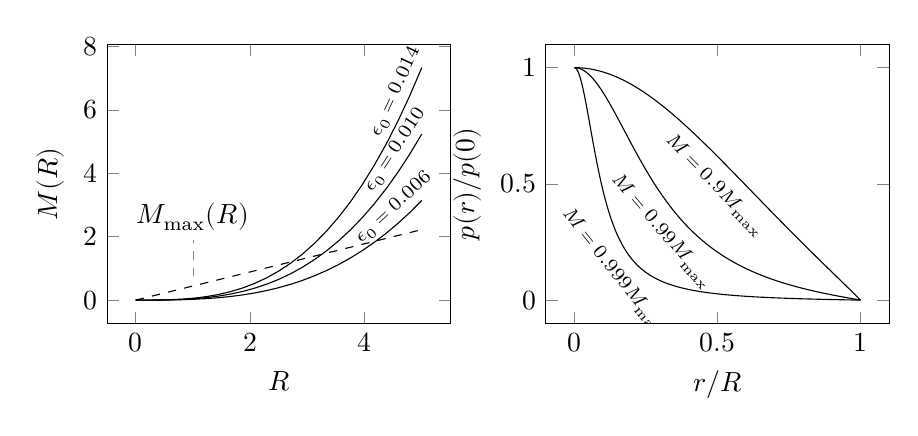
\begin{tikzpicture}
\begin{groupplot}[group style={group size=2 by 1, horizontal sep=0.1\textwidth}, width=0.49\textwidth]
	\nextgroupplot[xlabel=$R$, ylabel=$M(R)$, legend pos=north west, legend cell align=left, declare function={
		G = 1;
		M(\R,\E) = 4/3*pi*(\R)^3*\E;
		Mmax(\R) = 4*\R/(9*G);
	}]
	\pgfplotsinvokeforeach{0.014, 0.010, 0.006} {
		\addplot [domain=0:5, solid ] {M(x,#1)} node[pos=0.90, sloped, yshift=+5pt] {\scriptsize $\epsilon_0 = #1$};
	}
	\addplot [domain=0:5, dashed] {Mmax(x)} node[pos=0.2, pin=above:{$M_\text{max}(R)$}] {};
	%\legend{$M(R) = 4 \pi R^3 \epsilon_0 / 3$, $M_\text{max}(R) = 4R/9G$};
	\nextgroupplot[xlabel=$r/R$, ylabel=$p(r)/p(0)$, declare function={
		G=1;
		R=2;
		p(\r,\M) = \M / (4/3*pi*R^3) * (sqrt(1-2*G*\M*(\r)^2/R^3) - sqrt(1-2*G*\M/R)) / (3*sqrt(1-2*G*\M/R) - sqrt(1-2*G*\M*(\r)^2/R^3));
		Mmax = 4*R/(9*G);
	}]
	\pgfplotsinvokeforeach{0.9, 0.99, 0.999} {
		\addplot [domain=0:1,samples=200] {p(x*R,#1*Mmax)/p(0,#1*Mmax)} node[pos=0.5, sloped, yshift=-8pt] {\scriptsize $M = #1 M_\text{max}$};
	}
\end{groupplot}
\end{tikzpicture}
\caption{Mass-radius relation $M(R)$ for stars of density $\epsilon_0 = 0.01$ compared to the maximum supported mass $M_\text{max}$ and pressure distribution $p(r)$ for particular stars with density $\epsilon_0=0.01$, radius $R=2$ and different masses $M$ approaching $M_\text{max}$.}
\end{figure}

\appendix

\chapter{General relativity}
\section{Summary of important quantities}
\label{chap:gr_summary}

TODO: derive from Einstein-Hilbert action?

In general relativity, the geometry of spacetime is described by the \textbf{metric} $g\indices{_\mu_\nu}$ and the \textbf{line element}
\begin{equation}
	\dif s^2 = g\indices{_\mu_\nu} \dif x^\mu \dif x^\nu .
	\label{eq:def_line_elem}
\end{equation}

From the metric, we can construct the \textbf{Christoffel symbols}
\begin{equation}
	\Gamma^\sigma_{\mu \nu} = \frac{1}{2} g\indices{^\sigma^\epsilon} \left(
		\partial\indices{_\mu} g\indices{_\nu_\epsilon} +
		\partial\indices{_\nu} g\indices{_\epsilon_\mu} +
		\partial\indices{_\epsilon} g\indices{_\mu_\nu}
	\right) .
	\label{eq:def_christoffel}
\end{equation}

They allow us to generalize the partial derivative of a contravariant vector $V^\nu$ or a covariant vector $V_\nu$ to the \textbf{covariant derivative}
\begin{equation*}
	\nabla_\mu V^\nu = \partial_\mu V^\nu + \Gamma_{\sigma \mu}^\nu V^\sigma
	\qquad \text{or} \qquad
	\nabla_\mu V_\nu = \partial_\mu V_\nu - \Gamma_{\nu \mu}^\sigma V_\sigma
	.
\end{equation*}
For a general type $(r,s)$ tensor $T^{\alpha_1 \ldots \alpha_r}_{\beta_1 \ldots \beta_s}$ (where we suppress the order of the indices),
\begin{equation}
\begin{split}
	\nabla_\mu T^{\alpha_1 \ldots \alpha_r}_{\beta_1 \ldots \beta_s} &= \partial_\mu T^{\alpha_1 \ldots \alpha_r}_{\beta_1 \ldots \beta_s} \\
	                                                                 &+ \Gamma^{\alpha_1}_{\sigma\mu} T^{\sigma \alpha_2 \ldots \alpha_r}_{\beta_1 \ldots \beta_s} + \dots + \Gamma^{\alpha_r}_{\sigma\mu} T^{\alpha_1 \ldots \alpha_{r-1}\sigma}_{\beta_1 \ldots \beta_s} \\
	                                                                 &- \Gamma^\sigma_{\beta_1 \mu} T^{\alpha_1 \ldots \alpha_r}_{\sigma \beta_2 \ldots \beta_s} - \cdots - \Gamma^\sigma_{\beta_s \mu} T^{\alpha_1 \ldots \alpha_r}_{\beta_1 \ldots \beta_{s-1} \sigma}.
	\label{eq:def_cov_deriv}
\end{split}
\end{equation}
\iffalse
\begin{align}
	\nabla_c T\indices{^{a_1 \ldots a_r}_{b_1 \ldots b_s}} &= \partial_c {T^{a_1 \ldots a_r}}_{b_1 \ldots b_s} \\
	                                                       &+ \Gamma^{a_1}_{dc} T\indices{^{d a_2 \ldots a_r}_{b_1 \ldots b_s}} + \dots + \Gamma^{a_r}_{dc} T\indices{^{a_1 \ldots a_{r-1}d}_{b_1 \ldots b_s}} \\
	                                                       &- {\Gamma^d}_{b_1 c} {T^{a_1 \ldots a_r}}_{d b_2 \ldots b_s} - \cdots - {\Gamma^d}_{b_s c} {T^{a_1 \ldots a_r}}_{b_1 \ldots b_{s-1} d}.
	\label{eq:def_cov_deriv}
\end{align}
\fi
That is, for each upper index $\alpha_i$, add $+\Gamma^{\alpha_i}_{\sigma \mu} T^{\alpha_1 \ldots \alpha_{i-1} \sigma \alpha_{i+1} \ldots \alpha_r}_{\beta_1 \ldots \beta_s}$,
and for each lower index $\beta_i$, add $-\Gamma^{\sigma}_{\beta_i \mu} T^{\alpha_1 \ldots \alpha_r}_{\beta_1 \ldots \beta_{i-1} \sigma \beta_{i+1} \ldots \beta_s}$,
As the name and notation suggests, $\nabla_\mu$ transforms covariantly, so the covariant derivative of a tensor is independent of coordinate system.

The curvature of spacetime is expressed through the \textbf{Riemann curvature tensor}
\begin{equation}
	R\indices{^\epsilon_\sigma_\mu_\nu} =
	\partial\indices{_\mu} \Gamma^\epsilon_{\nu \sigma} -
	\partial\indices{_\nu} \Gamma^{\epsilon}_{\mu \sigma} +
	\Gamma^\epsilon_{\mu \lambda} \Gamma^{\lambda}_{\nu \sigma} -
	\Gamma^\epsilon_{\nu \lambda} \Gamma^{\lambda}_{\mu \sigma} .
	\label{eq:def_riemann_tensor}
\end{equation}

The curvature tensor can be contracted to form the \textbf{Ricci tensor}
\begin{equation}
	R\indices{_\mu_\nu} = R\indices{^\lambda_\mu_\lambda_\nu},
	\label{eq:def_ricci_tensor}
\end{equation}
whose trace is known as the \textbf{Ricci scalar}
\begin{equation}
	R = R\indices{^\mu_\mu} .
	\label{eq:def_ricci_scalar}
\end{equation}
For more details, consult an introductory textbook on general relativity like \cite{ref:carroll}.

\chapter{Code}

\section{Derivation of the Tolman-Oppenheimer-Volkoff equation \texorpdfstring{\\}{} without using energy-momentum conservation}
\label{sec:tov_cas_derivation}

When deriving \cref{eq:tov} analytically, we made use of energy-momentum conservation $\nabla_\mu T\indices{^\mu^\nu} = 0$ instead of substituting our results into the unused \cref{eq:einstein_to_tov:thetatheta}.
Here, we do the latter in the computer algebra system SAGE.

\inputminted{python}{../code/einstein_to_tov/ein.sage}

The output matches \cref{eq:tov} precisely.

\printbibliography

\end{document}
